\chapter{CSP (Constraint Satisfaction Problems}
It is often better to describe states in terms of features and then to reason in terms of these features and we have called this a \emph{factored representation}.

This representation may be more natural and efficient than explicitly enumerating the states, so with $10$ binary features we can describe $2^{10} = 1024$ states,
often these features are not independent and there are constraints that specify legal combinations of assignments of values to them.

A CSP is a problem composed of a finite set of variables, each variable is
associated with a finite domain and a set of constraints that restrict
the values of the variables can simultaneously take, so the task is to
assign a value (from the associated domain) to each variable 
satisfying all the constraints;
this problem is in NP hard in the worst cases but general heuristics exist, and structure can be exploited for efficiency.

A Constraint Satisfaction Problem consists of three components, $X, D,$ and $C$,
so $CSP = (X, D, C)$ where $X$ is a set of variables $\{x_1, \dots, x_n\}$, $D$ is a set of domains $\{D_1, \dots, D_n\}$, one for each variable, and 
$C$ is a set of contraints that specify allowable combinations of values.

A [partial] assignment of values to a set of variables (also called compound
label) is a set of pairs $A = \{(x_i, v_i), (x_i, v_j), \dots\}$
where values are taken from the variable domain and we have that a 
complete assignment is an assignment to all the variables
of the problem (a possible world).\newline
A complete assignment can be projected to a smaller partial assignment
by restricting the variables to a subset and we will use the projection operatorfrom relational algebra as notation.

A constraint on a set of variables is a set of possible assignments for 
those variables and each constraint C can be represented as a pair (scope, rel),where scope is a tuple of variables participating in the constraint 
$(x_1, x_2, \dots, x_k)$ and rel is a relation that defines the allowable 
combinations of values for those variables, taken from their respective domains.

To solve a CSP problem $(X, D, C)$, seen as a search problem, we need to 
define a state space and the notion of a solution:
a state in a CSP is an assignment of values to some or all of the variables and we have a partial assignment when we assigns values to only some of the variables, a complete assignment when every variable is assigned and in the end
a consistent assignment is the one that satisfies all the constraints.\newline
A solution to a CSP (a goal state) is a consistent, complete assignment.

The simplest kind of CSP involves variables that have discrete,
finite domains and values can be numbers, strings, Booleans (True, False);
when variables are numbers, and the constraints are inequalities we can deal
with variables with infinite domains or continuous domains with linear
or integer programming (techniques used in Operations research).

According to the number of variables involved constraints can be unary,
binary or higher-order constraints and there can be some preferences constraints
and that case we can solve using some optimization methods called 
\emph{Constraint Optimization Problems}.

Problem reduction/Constraint propagation are techniques for transforming
a CSP into an equivalent one which is easier to solve or recognizable
as insoluble (removing values from domains and tightening constraints) and 
we can elso exploits the structure of the problem as we will deal later.

We will majority consider CSP with unary and binary constraints only and 
a binary CSP may be represented as an undirected graph $(V, E)$, where $V$
correspond to variables and edges correspond to binary constraints among $V$.

We define that graph as \emph{Constraint graph} and also a node $x$ is adjacent
to node $y$ if and only if $(x, y) \in E$.

We can consider only binary CSP, since all problems can be transformed into 
binary constraint problems (not always worthwhile) using dual graph 
transformation where constraints became variables and if two constraints share
variables they are connected by an arc, correspondig to the constraint that
the shared variables receive the same value.

In general, every CSP is associated with a \emph{constraint hypergraph},
which are a generalization of graphs, so in a hypergraph a hypernode may
connect more than two nodes.

The constraint hypergraph of a CSP$(X, D, C)$ is a hypergraph in which each
node represents a variable in $X$ and each hyper-node represents a 
higher order constraint in $C$.

Reducing a problem means removing from the constraints those assignments which
appear in no solution tuples and we have that two CSP problems are equivalent
if they have identical sets of variables and solutions.

A CSP problem $P_1$ is reduced to a problem $P_2$ when $P_1$ is equivalent to
$P_2$, domains of variables in $P_2$ are subsets of those in $P_1$ and the 
constraints in $P_2$ are at least as restrictive than in $P_1$.

These conditions guarantee that a solution to $P_2$ is also a solution to $P_1$
and only redundant values and assignments are removed.

Problem reduction involves two possible tasks:
\begin{enumerate}
    \item removing redundant values from the domains of the variables. 
    \item tightening the constraints so that fewer compound labels satisfy them.
\end{enumerate}
Constraints are sets, so if the domain of any variable or any constraint
is reduced to an empty set, one can  conclude that the problem is
unsolvable.

Problem reduction is also called \emph{consistency checking} since it relies
on estabilishing local consistency properties, that are the following:
\begin{description}
   \item [Node Consistency:] a node is consistent if all the values in its 
	   domain satisfy unary constraints on the associated variable.
	
	   Node consistency is done using the algorithm called NC-1 that 
           has time complexity $O(dn)$.
   \item [Arc consistency:] a variable is arc-consistent if every value in 
	   its domain satisfies the binary constraints of this variable with
           other variables.\newline
	   $x_i$ is arc-consistent with respect to another variable $x_j$ if
	   for every value in its domain $D_i$ there is some value in the
     domain $D_j$ that satisfies the binary constraints on the arc $(x_i, x_j)$.

     	   The most popular algorithm for arc consistency is called AC-3, with
	   pseudocode visible in figure \ref{img:ac3}, and assuming a CSP with
	   $n$ variables, each with domain size at most $d$, and with $c$
	   binary constraints, each arc $(x_k, x_i)$ can be inserted in the 
	   queue only $d$ times since $x_i$ has at most $d$ values to delete
	   and checking consistency of an arc can be done in $O(d^2)$ so 
	   we get $O(cd^3)$ as total worst-case time.

	   \begin{figure}
		   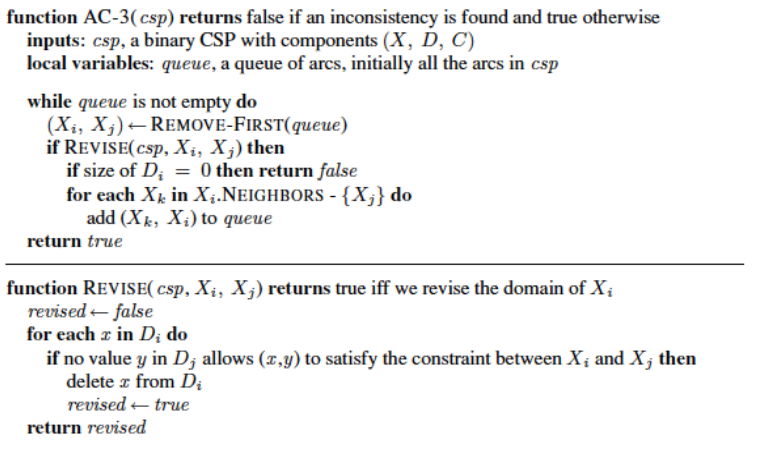
\includegraphics[width=0.8\textwidth]{Images/ac-3}
		   \caption{Pseudocode of $\proc{AC-3}$}
		   \label{img:ac3}
	   \end{figure}

          An improvement is provided by AC-4, based on the notion of support, 
	  that doesn't need to consider all the incoming arcs and yields to
	  $O(cd^2)$.
  \item [Forward Checking:] a very weak, local and quick form of consistency
	  which is triggered during the search process, so when we assign a 
	  value $v$ to a variable $x$ in the process of searching for a 
	  consistent assignment, we check the neighbor's variables and exclude
	  values that are not compatible with $v$ from their domains.

  \item [Generalized Arc Consistency: ] an extension of the notion of arc 
	  consistency to handle n-ary constraints and we says that a variable
	  $x_i$ is generalized arc consistent with respect to a n-ary constraint
	  if for every value $v$ in the domain of $x_i$ there exists a tuple
	  of values that is a member of the constraint and has its $x_i$ 
	  component equal to $v$.

	  The GAC algorithm is a generalization of AC-3 and it uses hypergraphs.
	
  \item [Path consistency: ] it tightens the binary constraints by using 
	  implicit constraints that are inferred by looking at triples of 
	  variables and a path of length $2$ between variables $x_i, x_j$
	  with respect to a third intermediate variable $x_m$ if, for every
	  consistent assignment there is an assignment to $x_m$ that satisfies
	  the constrains on $(x_i, x_m)$ and $(x_m, x_j)$; the algorithm
	  used is called PC-2 and Montanari says that if all path of length $2$
	  are made consistent, then all path of any length are consistent.

  \item [$k$-consistency:] a generalization of the other properties, so a CSP
	  is $k$-consistent if for any set of $k-1$ variables and for any 
	  constraint assignment to those variables, a consistent value can 
	  always be assigned to any $k$ variable.

  \item [Domain splitting: ] split a problem into a number of disjoint cases
	  and solve each case separately and the set of solutions to the 
	  initial problem is the union of the solutions to each case.
	
  \item [Variable Elimination: ] simplifies the network by removing variables
	  and we can eliminate $x$, having taken into account constraints
	  of $x$ with other variables and obtain a simpler network.
\end{description}

Problem reduction techniques are used in combination with search and in figure
\ref{img:reductionCost} is possible to note the cost of problem reduction 
and the cost of search, so we discover that more effort one spends on 
problem reduction the less effort one needs in searching.

\begin{figure}
	\centering
	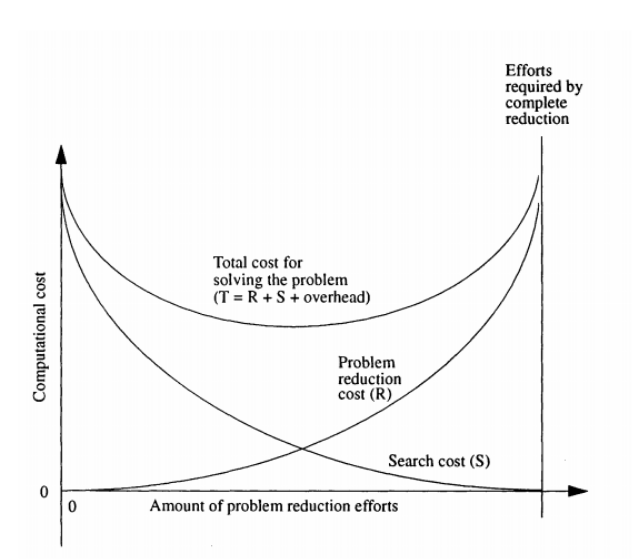
\includegraphics[width=0.6\textwidth]{Images/searchCost}
	\caption{Comparison of Search and Forward Checking cost in CSP problems}
	\label{img:reductionCost}
\end{figure}

Most problems cannot be solved by problem reduction alone, in this case we must
search for solutions or combine problem reduction with search.

In this context we talk about \emph{constraint propagation} and we can exploit
\emph{commutativity} since the order of variable assignment does not change
the result so we have only $d^n$ leaves instead of $n!d^n$.

To solve CSP we use the \emph{backtracking} search algorithm, which pseudocode
is visible in figure \ref{img:backtracking}, and we use some heuristics and 
search strategies that can be the following:
\begin{enumerate}
	\item To choose the next variable to assign we can use \emph{minimum-remaining-values} heuristic, which choose the variable with the fewest "legal" remaining values,
	     and \emph{degree heuristic}, which select the variable that is involved
	     in the largest number of constraints on other unassigned variables.

	\item To choose the value to assign we can use the \emph{Least-constraining-value}, which prefers the value that rules out the fewest choices for the neighboring 
	     variables in the constraint graph.

	\item To choose the inferences to perform at each step in the search we can
	      perform forward checking, which ensure arc consistency of last assigned 
	      variable, but we can also perform \emph{Mac} (Maintaining Arc Consistency)
	      where calls AC-3 but start with only the arcs $(X_j, X_i)$ for all
	      $X_j$ that are unassigned variables that are neighbors of $X_i$.
        \item To choose which variable to backtrack we can use \emph{chronological} 
	      backtracking, where we backtrack to previous variables that sometimes
	      is not useful to solve the problem, so we can use an "intelligent" 
	      way that is the \emph{Conflict backjumping}, that consist to find the 
	      variable responsible for the violation of constraints, using the 
	      \emph{conflict set}.

	      The rule for computing the conflict set is:
	      \begin{defi}
		  If every possible value for $X_j$ fails, backjump to the most recent
		  variable $X_i \in conf(X_j)$ and update its conflict set
		  \[ conf(X_i) = conf(X_i) \cup conf(X_j) - \{X_i\} \]
	      \end{defi}
	      \emph{Constraint learning} is the idea of finding a minimum set of 
	      variables from the conflict set that causes the problem and this set
	      of variables is called a \emph{no-good}.
\end{enumerate}

\begin{figure}
	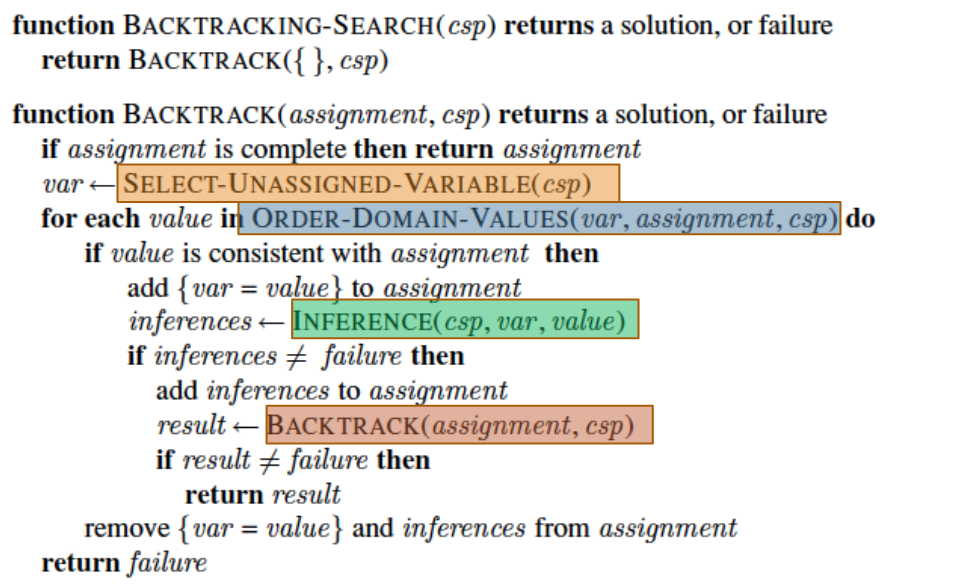
\includegraphics[width=0.8\textwidth]{Images/backtracking}
	\caption{Pseudocode of Backtracking algorithm}
	\label{img:backtracking}
\end{figure}

\section{Review of local search methods}
Local search methods require a complete state formulation of the problem:all the 
elements of the solution in the current state, so for CSP a complete assignment.

They keep in memory only the current state and try to improve it, iteratively and 
do not guarantee that a solution is found even if it exists,
so cannot be used to prove that a solution does not exist.

To be used when the search space is too large for a systematic search 
and we need to be very efficient in time and space, we need to provide a solution
but it is not important to produce the set of actions leading to it (the solution path)
and we know in advance that solutions exist.

In figure \ref{img:localSearch} is possible to note a generic algorithm for local 
search in CSP and we have some extreme cases:
\begin{description}
    \item [Random sampling: ] no walking is done to improve solution, so stop\_walk
	    is always true, just generating random assignments and testing them.
    \item [Random walk: ] no restarting is done ( stop\_walk is always false).
\end{description}

\begin{figure}
	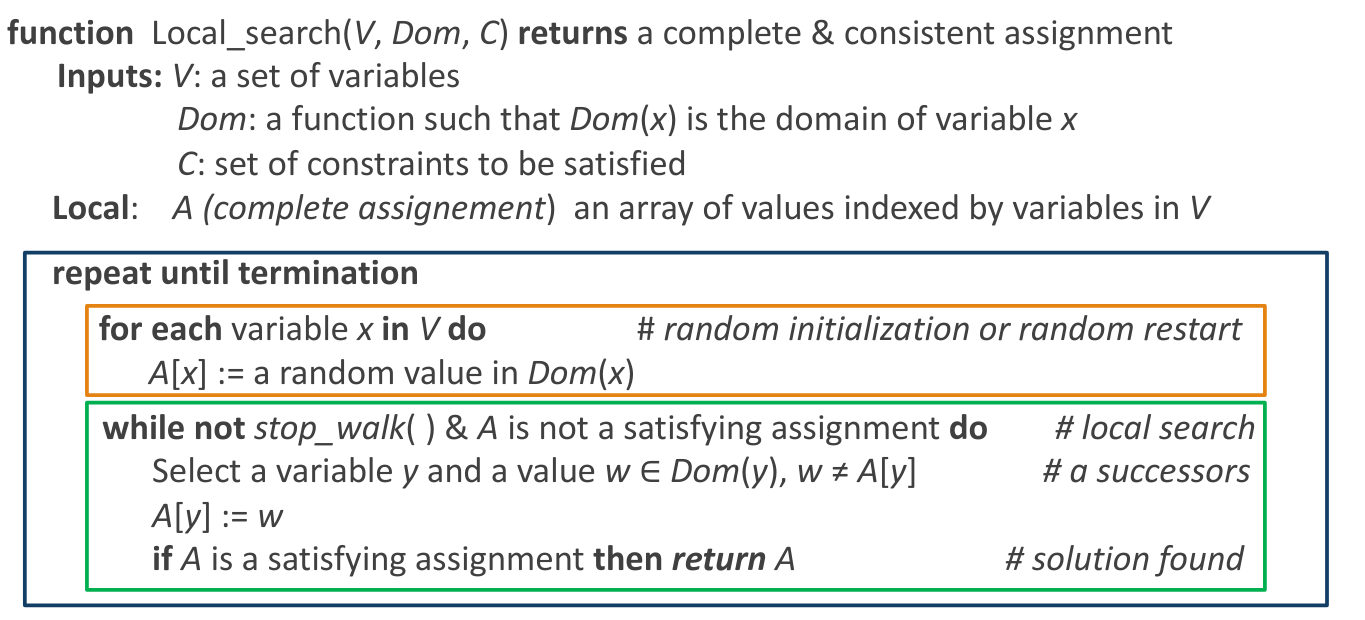
\includegraphics[width=\textwidth]{Images/genericLocalSearch}
	\caption{Pseudocode for a generic Local Search algorithm}
	\label{img:localSearch}
\end{figure}

We can inject heuristics in the selection of the variable and the value by means of
an evaluation function and in CSP we use $f = $number of violated constraints 
or conflicts (perhaps with weights), which we stop when $f = 0$.

Iterative best improvement consist to choose the successor that most improves 
the current state according to an evaluation function $f$ (greedy ascent/descent)
and if more than one we choose at random.

Hill-climbing stops when no improvement is possible and it can be stuck in local maxima
instead iterative best improvement algorithms move to the best successor, 
even if worse than current state and they may be stuck in a loop, so is not complete.

\emph{Stochastic local search} combine iterative best improvement with randomness,
which can be used to escape local minima, and we can use $2$ different type of random:
\begin{description}
    \item [Random restart:] is a global random move, where the search start from a 
	    completely different part of the search state.
    \item [Random walk: ] is a local random move, where random steps are taken 
	    interleaved with the optimizing steps.
\end{description}
All the local search techniques are candidates for application to CSPs, but 
\emph{Min-conflict heuristics} is widely used that consist to select a variable at
random among conflicting variables and then we select the value that results in the 
minimum number of conflicts with other variables.

The pseudocode of Min-conflict algorithm is visible in figure \ref{img:min_conflict}
and we have that the run time of min-conflict is roughly independent of problem size.

\begin{figure}
	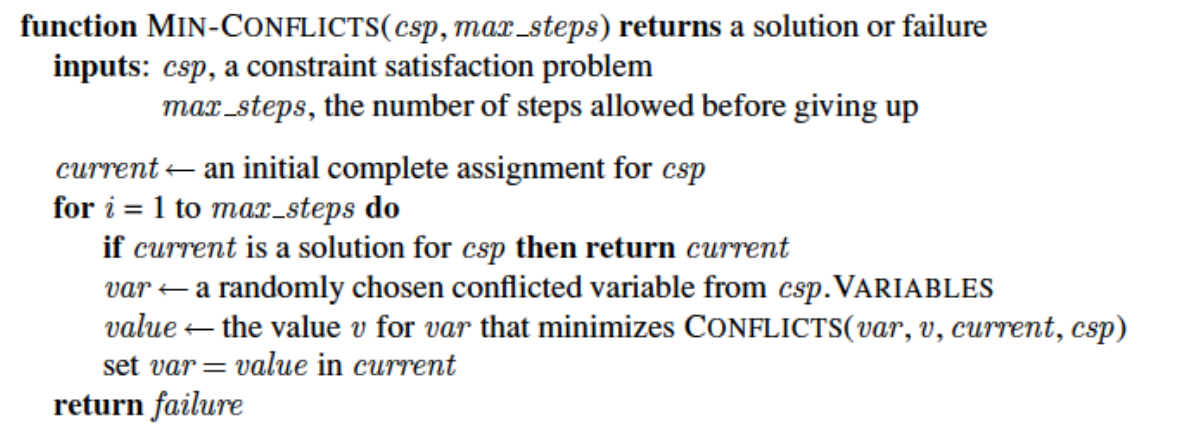
\includegraphics[width=\textwidth]{Images/min-conflicts}
	\caption{Pseudocode of Min-conflicts}
	\label{img:min_conflict}
\end{figure}

The landscape of a CSP under the min-conflict heuristic usually has a series of 
plateaux and possible improvements are:
\begin{description}
    \item [Tabu Search: ] local search has no memory, so the idea is keeping a small
	    list of the last $t$ steps and forbidding the algorithm to change the value
	    of a variable whose value was changed recently.
    \item [Constraint weighting: ] can help concentrate the search on the important
	    constraints and we assign a numeric weight to each constraint, which
            is incremented each time the constraint is violated.
    \item [Simulated annealing: ] is a technique for allowing downhill moves at the 
	    beginning of the algorithm and slowly freezing this possibility as the 
	    algorithm progresses.
    \item [Population based methods: ] inspired by biological evolution like 
	    genetic algorithms, \emph{local beam search}, which proceed with the 
	    best $k$ successors according to the evaluation function and also
	    \emph{stochastic local beam search} selects $k$ of the individuals at
	    random with a probability that depends on the evaluation function.
\end{description}
Another advantage of local search methods is that they can be used in an online 
setting when the problem changes dynamically, but randomized algorithms are difficult
to evaluate since they give a different result and a different execution time each
time they are run, so we have to take \emph{average/median runtime} but this definition
is ill defined since in case of algorithms that never ends we can't evaluate it.

\section{The Structure of Problems}
The structure of the problem reflects in properties of the constraint graph and 
when problems have a specific structure, we have strategies for improving the process
of finding a solution.

A first obvious case is that of \emph{independent subproblems}, so each connected
components of the constraint graph corresponds to a subproblem $CSP_i$, so if 
assignment $S_i$ is a solution of $CSP_i$, then $\cup _i S_i$ is a solution of 
$\cup_i CSP_i$.

This can save dramaticly computation time so we can solve CSP in $O(d^c n/c)$ linear
on the number of variables $n$ rather than $O(d^n)$ which is exponential.

If we can estabilish a total ordering of the variables we can compute a weaker form
of consistency called Directional Arc Consistency, and this property is less expensive
to compute, but in addition we need to solve a CSP problem when the shape of its 
constraint graph is a tree.\newline
A CSP is Directional Arc Consistent (DAC) under an ordering of the variables if and
only if for every label $(x, a)$, which satisfies the constraints on $x$, there exists
a compatible label $(y, b)$ for every variable $y$, which comes after $x$ according to
the ordering.\newline
In the algorithm for estabilishing DAC (DAC-1), each arc is examined exactly once by
proceedings from the last in the ordering, so the complexity is $O(cd^2)$.

In a tree-structured constraint graph two nodes are connected by only one path and 
we can choose any variable as the root of tree and chosen a variable as the root,
the tree induces a topological sort on the variables.

A CSP is defined to be directed arc-consistent under an ordering of variables $X_1, 
X_2, \dots, X_n$ if and only if every $X_i$ is arc-consistent with each $X_j$ for $j>i$.

We can make a tree-like graph directed arc-consistent in one pass over the $n$ variables
and each step must compare up to $d$ possible domain values for two variables $d^2$
for a total time of $O(nd^2)$.

\begin{figure}
	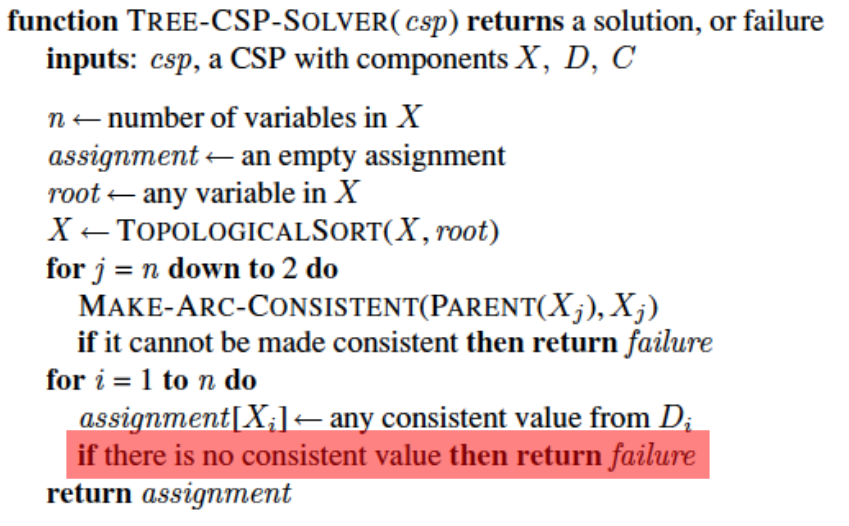
\includegraphics[width=0.8\textwidth]{Images/tree-CSP-Solver}
	\caption{Pseudocode for Tree CSP Solver}
	\label{img:treeSolver}
\end{figure}
To solve a tree-constraint graph for CSP we use the pseudocode in figure 
\ref{img:treeSolver}, and to make a graph in a Tree for CSP we have the following
two heuristics:
\begin{description}
    \item [Cutset conditioning: ] in general we must apply a domain splitting strategy,
	    and we choose a subset $S$ on the CSP's variables such that the constraint
	    graph becomes a tree after removal of $S$ ($S$ is called a \emph{cycle cutset}).

	   For each possible consistent assignment to the variables in $S$, we remove
	   the domains of the remaining variables any values that are inconsistent 
	   with the assignment for $S$ and if the remaining CSP has a solution
	   we return it together with the assignment for $S$.

	  With this approach we have $O(d^c (n-c)d^2)$ time complexity, where $c$ is
	  the size of the cycle cutset and $d$ is the size of the domain.
   \item [Tree decomposition: ] this appraoch consists in a tree decomposition of the 
	   constraint graph into a set of connected sub-problems and each sub-problem
	   is solved independently, and the resulting solutions are then combined.
	
	A tree decomposition must satisfy the following three requirements:
	\begin{enumerate}
	   \item Every variable in the original problem appears in at least of one 
		 of the sub-problems.
	   \item If two variables are connected by a constraint in the original problem,
		 they must appear together in at least one of the sub-problems.
	   \item If a variable appears in two sub-problems in the tree, it must
		 appear in every subproblem along the path connecting those 
		 those sub-problems.
	\end{enumerate}
\end{description}
\emph{Simmetry} is an important factor for reducing the complexity of CSP problems, and 
we have that \emph{Value simmetry}, which the value does not really matters, instead
in \emph{Symmetry-breaking constraints} we might impose an arbitrary ordering constraint,
that requires the three values to be in alphabetical order and in practice 
breaking value symmetry has proved to be important and effective on a wide range 
of problems.


